\chapter{Background}\label{Background}

\section{Automatic Music Transcription}

In general, transcription refers to the process of retrieving information from audible data, such as sounds or music. Specifically when applied on music, the information we seek is often an annotation in music notation. This is what is referred to as \textit{music transcription}. Generally, transcribing a musical piece is expensive, requiring both extensive experience within a specific instrumental field, as well as a lot of manual, time-consuming work. Early on in 1986, Martin Piszczalski stated that \textit{"The learned, human skill of transcribing music is one of the most sophisticated auditory-based pattern-recognition tasks that humans perform."}~\cite{10.5555/15202}. A decade prior he helped introduce the term \acrfull{AMT} covering a field in which now, many years later, has evolved significantly~\cite{piszczalski1977automatic}.

\subsection{Transcription using Deep learning}
Currently, the majority of state-of-the-art within \gls{AMT} utilizes deep learning~\cite{8350302, signals4040042, jamshidi2024machine}. With enough data one can train a \gls{DNN} to, given an input sequence of music, automatically output a transcribed sequence representing musical notation. Musical notation such as this could be extensive in their information, but by far the most important parts could be reduced down to \textit{"which instruments are playing"} and \textit{"when are they playing"}.

Relating this to a common deep learning task, this could be described as a multi-label sequence tagging/sequence labelling task. For each element in an input sequence output a combination of one or more labels. Each element within this sequence represents a timestep in the audio recording, with a combination of labels representing one or more instruments being played. This constitutes the most basic form of \gls{AMT}.

\begin{figure}[H]
    \centering
    \begin{tikzpicture}

\node[
    label=north:{\large{Music}}
] (music) at (-5.5, 0) {
    \begin{tikzpicture}
        \node at (0, 0) {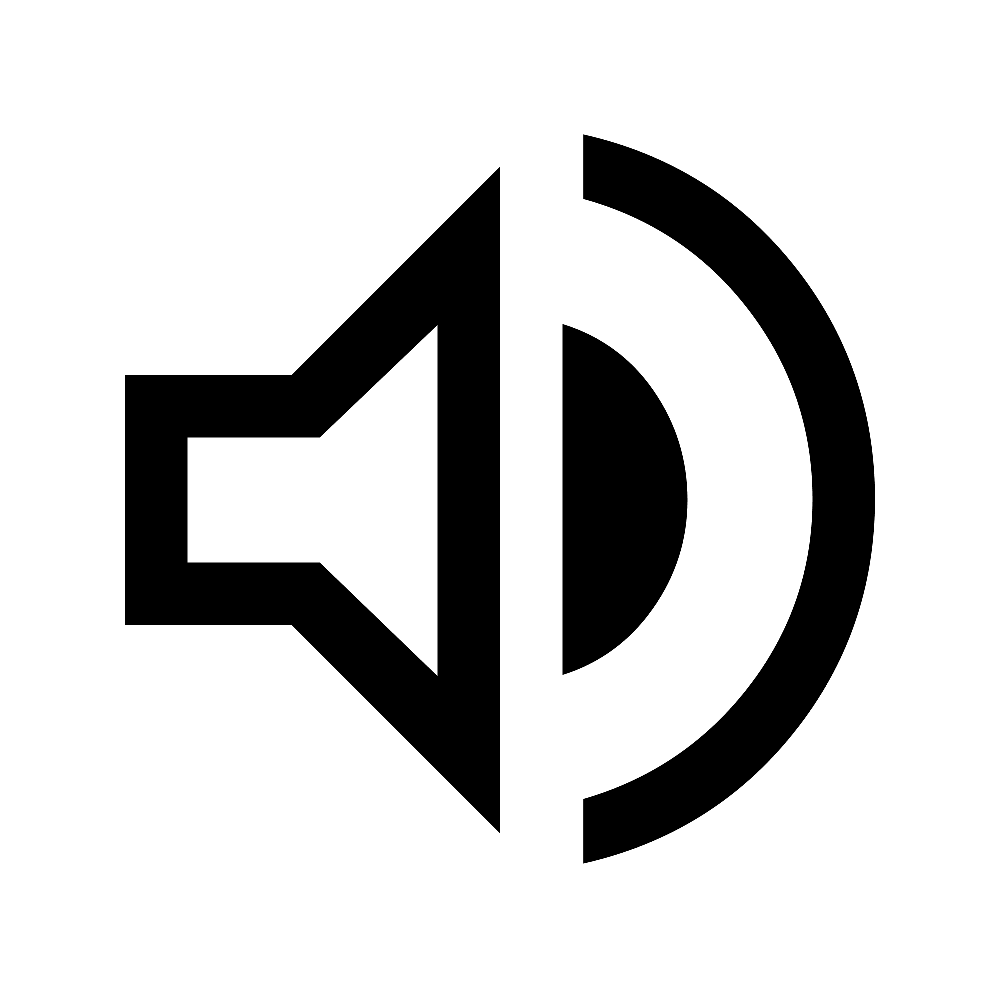
\includegraphics[scale=0.06]{figures/speaker.png}};
        \node [rotate=30, scale=1.6] at (1.1, 0.85) {\AAcht};
        \node [rotate=-30, scale=1.2] at (1, -0.75) {\Acht};
    \end{tikzpicture}
    };

\node[
    label={[label distance=1.08em]north:{\large{Deep Learning}}},
    rectangle,
    draw,
    thick,
    minimum height=5em,
    minimum width=10em,
] (nn) at (0, 0) {\large{Neural Network}};

\node[
    label={[label distance=1.08em]north:{\large{Transcription}}},
    minimum height=5em,
] (transcription) at (5.5, 0) {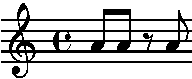
\includegraphics[scale=1.0]{lilypond/amt.cropped.pdf}};

\draw[->, thick] (music.east) -- (nn.west);
\draw[->, thick] (nn.east) -- (transcription.west);

\end{tikzpicture}

    \caption{An abstract visualization of the \acrfull{AMT} process using deep learning. Music is input, processed by a neural network, and ultimately converted into a symbolic transcription.}
    \label{AMTFigure}
\end{figure}

\section{Audio}

Sound is described by \textit{"the sensation caused in the nervous system by vibration of the delicate membranes of the ear."}~\cite{1953fundamentals}. In short, sound is the human perception of acoustic waves in a transition medium, like air. These waves, consisting of vibrating molecules, get sensed by our auditory organs and perceived by the brain. 

Thus sound can be described as the propogation and perception of waves. Mathematically, waves can be studied as signals~\cite{8454362}. To represent these sounds digitally, as \textit{audio}, one can express these waves as a signal, giving rise to the \textit{waveform}. The waveform is a timewise representation of a signal as a graph, charting the amplitude, or strength of the signal, over time.

\begin{figure}[H]
    \centering
    \begin{tikzpicture}

% Waveform signal
\draw[
domain=0:9, 
samples=300,
smooth,
variable=\x,
blue,
ultra thick,
shift={(-4.5, 2.2)},
] plot ({\x},{sin((3.05*\x + 0.3) r) * 0.8});
\node at (0, 3.5) {\large Digital Waveform};
    
% Pressure wave
\node[
    label=south:{\large Acoustic Sound Wave}
] (pressure) at (0, 0) {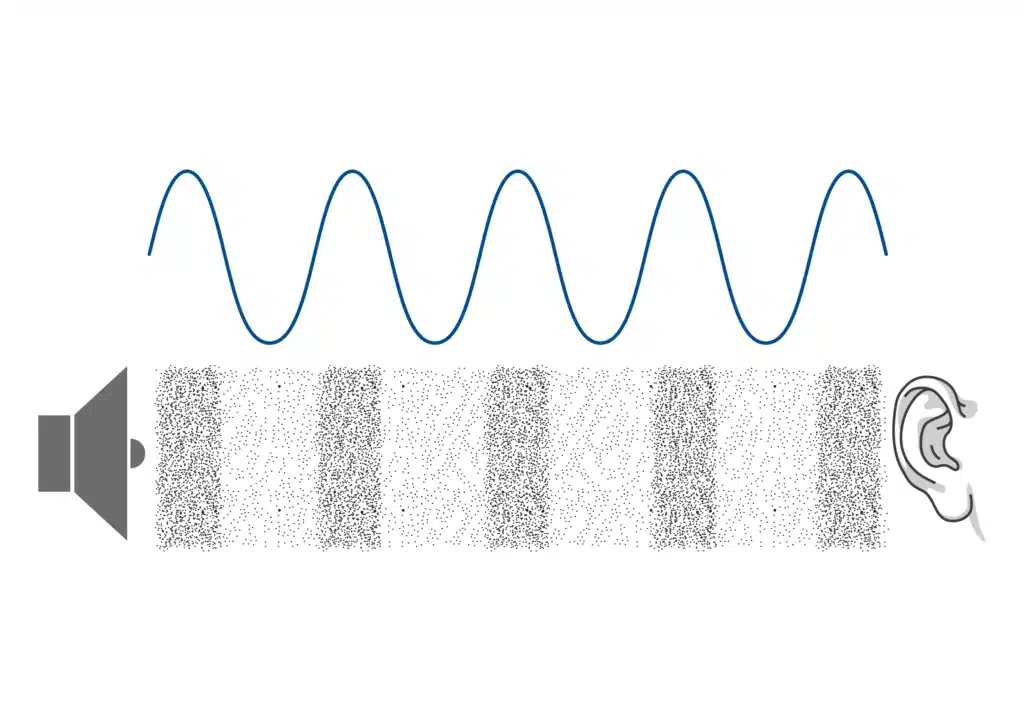
\includegraphics[trim={5.25cm 5.5cm 4.75cm 12.5cm},clip,scale=0.35]{figures/waveform}};

% Speaker
\node[left=-0.25cm of pressure] {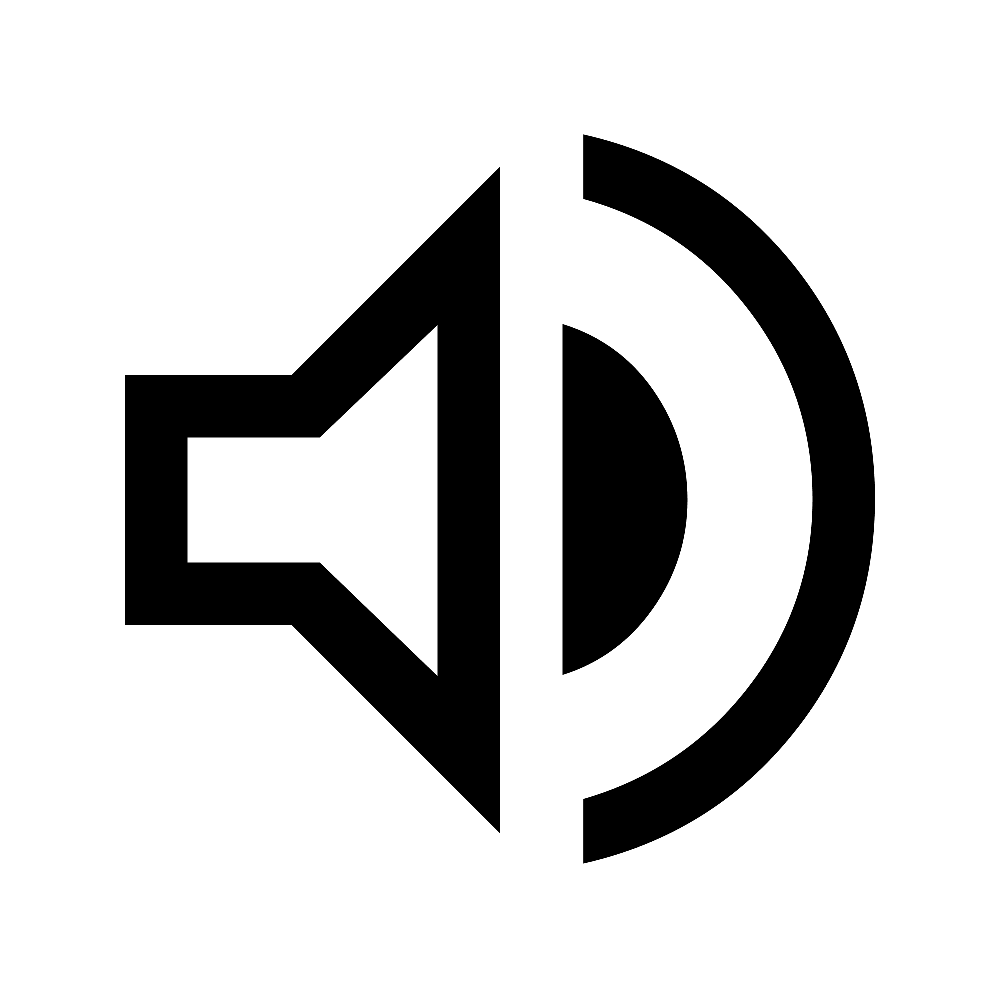
\includegraphics[scale=0.065]{figures/speaker.png}};

% Ear
\node[right=-0.25cm of pressure] {\scalebox{-1}[1]{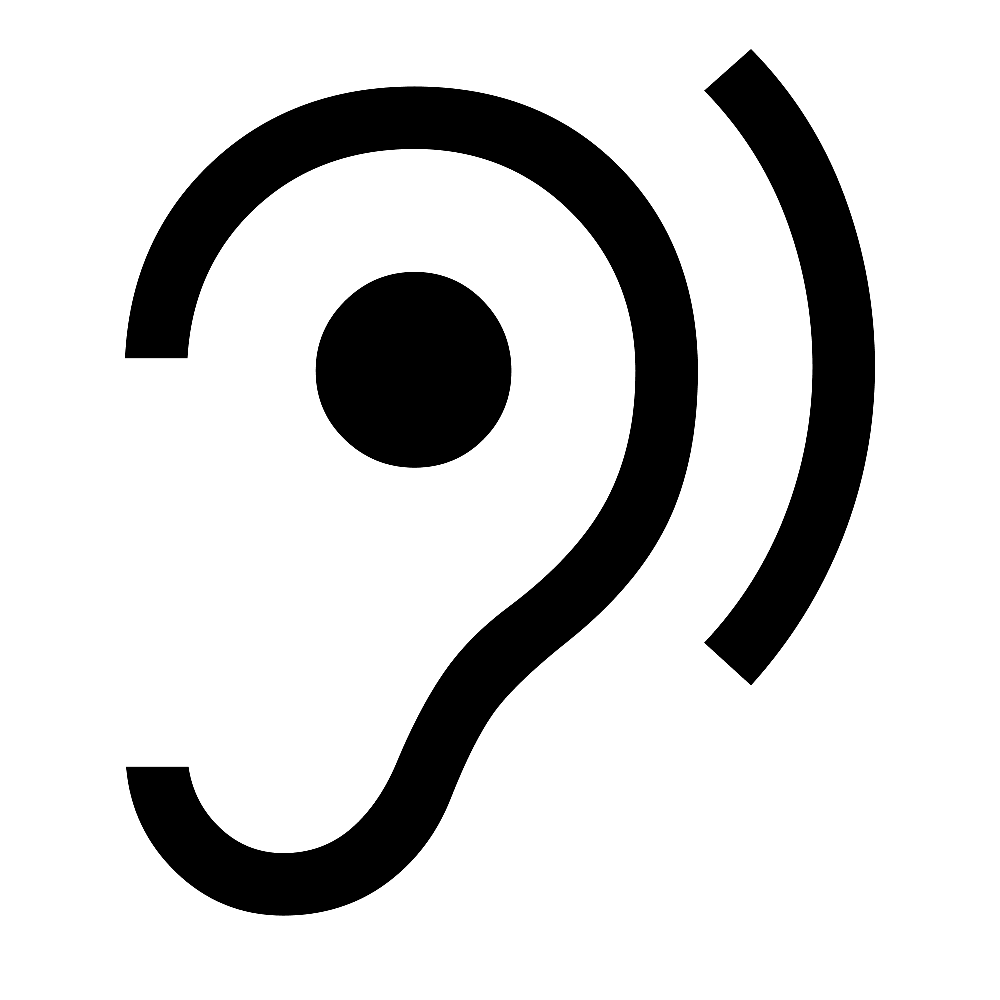
\includegraphics[scale=0.065]{figures/ear.png}}};

\end{tikzpicture}
    \caption{The relationship between an acoustic sound wave and its corresponding digital waveform. The waveform represents variations in the air pressure over time. Regions of higher and lower pressure in the sound wave correspond to \textit{peaks} and \textit{troughs} in the waveform, respectively.}
    \label{WaveformFigure}
\end{figure}

For monophonic sound, this waveform is a one-dimensional representation. Even though this is an excellent way of storing audio digitally, informationally it is very dense. Although there do exist deep learning models working directly with these waveforms, such as Oord et al.'s WaveNet~\cite{oord2016wavenetgenerativemodelraw}, the task of parsing and perceiving such a signal is a complex one. Luckily, there exists some processing techniques which can be applied to a waveform, lowering its complexity whilst keeping information intact.

\subsection{Fourier Transform}

The Fourier Transform is a mathematical transformation which, given a signal and frequency, computes the frequency's significance, or intensity, in the original signal. As we've established, audio is represented as a signal, meaning we therefore can use this transform, turning an audio signal into frequency space. 

The fourier transform is a complex transformation. Specifically given a signal $f$, we can compute the integral \[ \widehat{f}(\xi) = \int^{\infty}_{-\infty}{f(x)e^{-i2\pi \xi x} dx} \] for a frequency $\xi \in \mathbb{R}$, computed over all values $x \in \mathbb{R}$ representing time, resulting in a \textit{complex} number on the form $\widehat{f}(\xi) = a + bi$. This number consists of a \textit{real} part $a$ and an \textit{imaginary} part $b$. We can represent this complex number in polar form \[ a + bi = re^{i\theta}, \] where $r = \sqrt{a^2 + b^2}$ denotes the magnitude (amplitude) and $\theta = \arctan{(\frac{b}{a})}$, adjusted for the right quadrant, computes the phase of the respective frequency in the original signal $f$. Frequencies with higher amplitudes play a more prominent role in shaping the original sequence, indicating a greater significance. This information is what allow us to figure out which frequencies a signal is made out of and how each frequency contributes. 

By doing such a transform we turn our temporal data, like a waveform, into spectral data, its \textit{spectrum}. This inuitively \textit{untangles} our signal into its respective base frequencies. By ridding our data with the highly dense temporal aspect, replacing it with a more informationally independent and sparse spectral representation, a transformation such as this could lessen the complexity of the task, making the audio easier to \textit{understand}; in a metaphorical sense.

\begin{figure}[H]
    \centering
    \hspace*{-1.3cm}
    \begin{tikzpicture}
        \node at (0, 0) {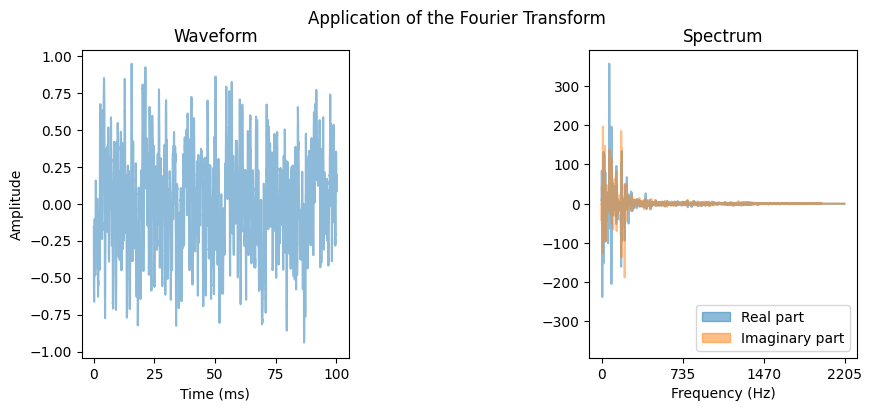
\includegraphics[scale=0.8]{figures/fouriertransform}};
        \draw[->] (-1, 0) -- (1.75, 0) node[above, midway, font=\footnotesize] {Fourier Transform};
    \end{tikzpicture}
    \caption{The Fourier Transform decomposes a waveform into its frequency components. The time-domain waveform signal on the left is measured in amplitude, where higher amplitudes correspond to higher sound wave air pressure levels. The frequency-domain spectrum on the right displays the amplitude of each frequency, indicating its contribution to the original signal.}
    \label{FTFigure}
\end{figure}

Note that the Fourier Transform is invertible, meaning that the original signal can be reconstructed from its frequency components via an inverse transformation. This property is fundamental to the Fourier Transform's integral and widely exploited within signal processing.

\subsection{Discrete Fourier Transform}

The Fourier Transform is defined as an integral over continuous time. On computers, instead of storing signals continuously we instead store signals using a discrete number of samples. Each signal's \textit{sampling rate} describes how many samples a signal contains per second of audio, and is denoted in \textit{Hz}.

To extract frequency values from these signals, we instead have to use the \gls{DFT}. Intuitively this works identically to the normal Fourier Transform, just ported to work on discretely sampled signals. It is given by the formula \[ X_k = \sum^{N - 1}_{n=0}{x_n \cdot e^{-i 2\pi \frac{k}{N} n}}, \] where $k$ denotes a certain frequency bin and $N$ the number of discrete samples. Note that contrary to the normal Fourier transformer, instead of computing the magnitude of each specific real-valued frequency, we instead compute the magnitude of frequencies covered by certain frequency bins. The number, or granularity, of these bins are directly dependent on the number of samples $N$, and the respective frequencies covered by each bin is given by the signal's sampling rate.

\subsection{Nyquist frequency}

When a continuous signal, such as an audio wave traveling through the air, is discritized by recording it on a computer, some information may be lost in the process. The discrete representation of the signal is an \textit{approximation} which quality is directly dependent on the sampling rate. The higher the sampling rate, the \textit{closer} we are to the original, continuous signal. However a higher sampling rate comes at the cost of needing to store these signals at a higher precision. A lower sampling rate would need less information stored, but this could also mean a less precise signal approxmation.

\textit{Aliasing} is the phenomenon where new, incorrect frequencies emerge in undersampled signals. The \textit{Nyquist frequency}, defined as half the sampling rate, represents the highest frequency that can be accurately captured by a discrete signal. Thus to prevent aliasing, the sampling rate must be at least twice the maximum frequency present in the original signal.

\begin{figure}[H]
    \centering
    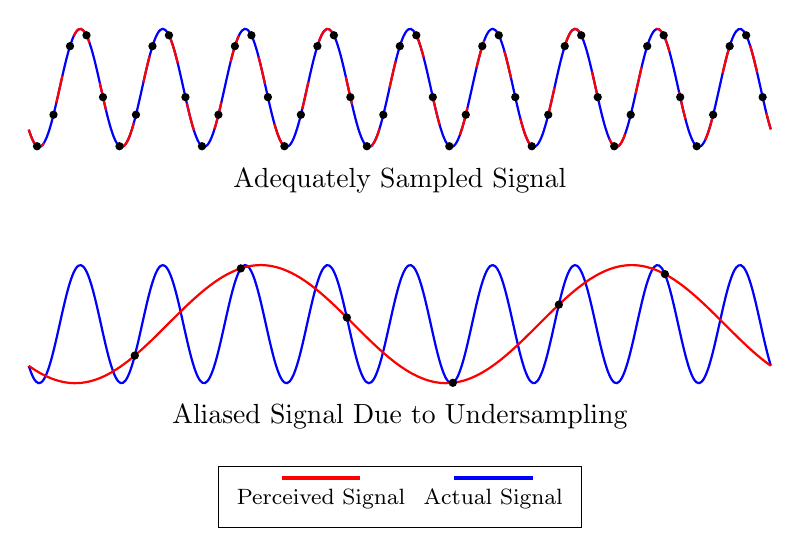
\begin{tikzpicture}[scale=1.5]

% Above Signal
\draw[
domain=0:2*pi, 
samples=300,
smooth,
variable=\x,
blue,
thick,
shift={(0, 2)}
] plot ({\x},{sin((9*\x - 3*pi/4) r)/2});

% Above Perceived
\draw[
domain=0:2*pi, 
samples=300,
smooth,
variable=\x,
red,
thick,
dash pattern={on 10pt off 15pt},
shift={(0, 2)}
] plot ({\x},{sin((9*\x - 3*pi/4) r)/2});

% Scatter Adequate Samples
\foreach \i in {1,...,45} {
    \pgfmathsetmacro\xsamp{2*pi*(\i-0.5)/45}
    \pgfmathsetmacro\ysamp{sin((9*\xsamp - 3*pi/4) r)/2}
    \fill (\xsamp, \ysamp + 2) circle (1pt);
}

% Above Text
\node[
anchor=north, 
] at (pi, 1.4) {Adequately Sampled Signal};


% Below Signal
\draw[
domain=0:2*pi, 
samples=300,
smooth,
variable=\x,
blue,
thick
] plot ({\x},{sin((9*\x - 3*pi/4) r)/2});

% Below Perceived
\draw[
domain=0:2*pi, 
samples=100,
smooth,
variable=\x,
red,
thick
] plot ({\x},{sin((2*\x - 3*pi/4) r)/2});

% Scatter Aliasing Samples
\foreach \i in {1,...,6} {
    \pgfmathsetmacro\xsamp{2*pi*\i/7}
    \pgfmathsetmacro\ysamp{sin((9*\xsamp - 3*pi/4) r)/2}
    \fill (\xsamp, \ysamp) circle (1pt);
}

% Below Text
\node[
anchor=north, 
] at (pi, -0.6) {Aliased Signal Due to Undersampling};


% Legend
\tikzset{
    legend entry/.pic={
        \draw[pic actions, line width=1.5pt] (-0.5, 0) -- (0.5, 0);
    }
}
\matrix [draw, below] at (pi, -1.2) {
    \pic[red]{legend entry}; &  \pic[blue]{legend entry}; \\
    \node[font=\footnotesize] {Perceived Signal}; &  \node[font=\footnotesize] {Actual Signal}; \\
};

\end{tikzpicture}
    \caption{Example of aliasing due to undersampling. The original signal has a true frequency of 9~Hz. In the upper plot, sampling at a sufficiently high rate of 45~Hz allows the signal to be perceived and reconstructed accurately. In the lower plot, however, a lower sampling rate of 7~Hz causes aliasing, and the signal is incorrectly perceived as having a frequency of 2~Hz.}
    \label{AliasingFigure}
\end{figure}

In the case of the \gls{DFT}, it directly follows that the maximum frequency from which accurate information can be extracted is proportional to the signal's sampling rate. Specifically, it is equal to the signal's Nyquist frequency.

\subsection{Fast Fourier Transform}

Keen-eyed computer scientists may note that the \gls{DFT} has a time complexity of $\mathcal{O}(n^2)$, since it requires summing over $N$ values for each of the $N$ different frequencies. As a result, the \gls{DFT} scales poorly in regards to input size. For instance, given that the standard audio sampling rate is $44.1 \text{kHz}$, the computational cost becomes significant, making the \gls{DFT} impractical for real-time or large-scale signal analysis~\cite{pras2010sampling}.

The \gls{FFT} algorithm addresses this limitation by computing the same result as the \gls{DFT}, but with a time complexity of $\mathcal{O}(n\log{n})$ instead. Described by Gilbert Strang as \textit{"the most important numerical algorithm of our lifetime"}~\cite{strang1993wavelet}, the \gls{FFT} effectively solves the prior scaling problem, allowing us to efficiently extract spectral information from a signal even at high sampling rates.

There exist several different implementations of the \gls{FFT}. Among them, the Cooley–Tukey algorithm is by far the most widely used, and optimizes its calculations through a \textit{divide and conquer} approach, reducing redundant computation by reusing intermediate results~\cite{d3ea2d52-5ab2-3128-8b80-efb85267295d}.

\subsection{Short-time Fourier Transform}

The Fourier Transform comes with certain limitations; most notably in how, by transforming a signal into the frequency domain, we lose its temporal structure. Although this loss of time information may be acceptable for certain tasks, it poses a challenge for applications like music transcription and \gls{ADT} where timing of events is vital. So far, we've seen how the Fourier Transform unravels the frequency content of a signal as a whole. But what happens if we had applied it to smaller, localized partitions of the signal instead?

This leads us to the \gls{STFT}. Rather than transforming the entire signal at once, the \gls{STFT} applies the Fourier Transform to smaller, overlapping \textit{windows} of the signal. This allows us to extract frequency information while preserving much of its temporal resolution. The result is a two-dimensional representation, revealing the intensity of different frequencies over time.

\begin{figure}[H]
    \centering
    \begin{tikzpicture}

% Signal
\node[
    %label=north:{\Large{Application of the Short-Time Fourier Transform}},
    label=east:{\Huge{\textbf{\dots}}},
    label={[label distance=0.6cm]west:{\large{Signal}}}
] (signal) at (0, 0) {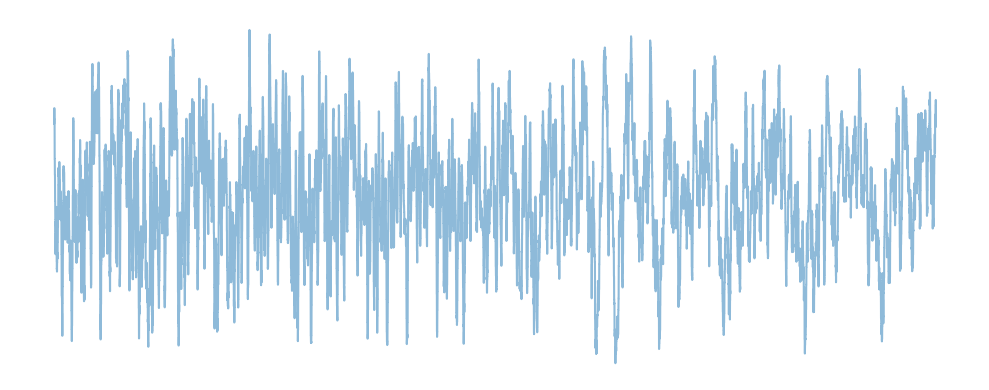
\includegraphics[scale=0.42]{figures/stftfull}};


% Window
\node[
    label=east:{\Huge{\textbf{\dots}}},
    label=west:{\large{Windows}},
    below=0.3cm of signal,
    xshift=-0.2cm
] (windows) {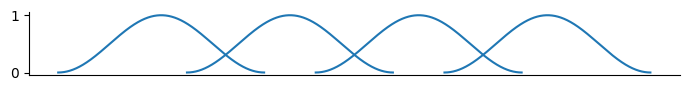
\includegraphics[scale=0.62,trim={0 0.25cm 0 0.2cm},clip]{figures/stftwindows}};

% Window Arrows
\draw[<->] ($(windows.north west) + (1.05, 0)$) -- ($(windows.north) - (1.25, 0)$) 
node[above, midway] (windowlabel) {\footnotesize{Window Length}};
\draw[<->] ($(windows.south west) + (1.05, 0)$) -- ($(windows.south) - (2.5, 0)$) 
node[below, midway] {\footnotesize{Hop Length}};


% Windows
\node[
    below=2cm of windowlabel
] (window0) {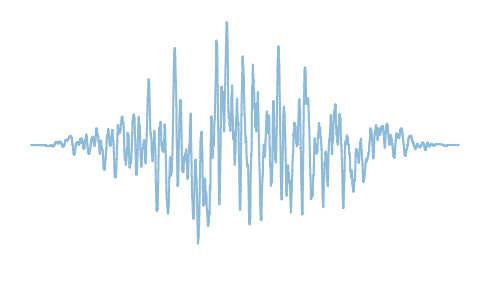
\includegraphics[scale=0.35]{figures/stftwindow0}};
\node[
    below right=-1.75cm and -1.8cm of window0,
    label={[label distance=3cm]west:{\parbox{2.5cm}{\centering \large{Window \\ Partitioning}}}}
] (window1) {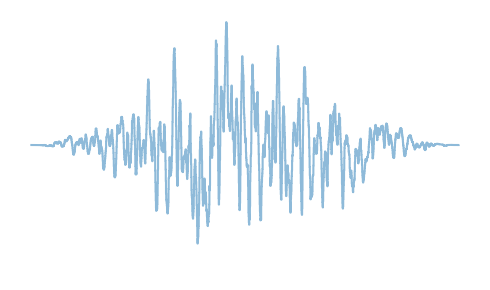
\includegraphics[scale=0.35]{figures/stftwindow1}};
\node[
    below right=-1.75cm and -1.8cm of window1,
    label={[rotate=-45]south east:{\Huge{\textbf{\dots}}}}
] (window2) {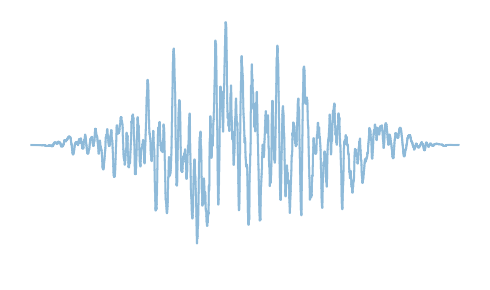
\includegraphics[scale=0.35]{figures/stftwindow2}};


% FFTs
\coordinate (fftarrow) at ($(window1.west |- window2.north) + (0, -1)$);
\draw[->, thick] (fftarrow) -- ($(fftarrow) + (0, -2.45)$) node[left, midway] {\large{FFT}};

\node[
    label=east:{\Huge{\textbf{\dots}}},
    below=1.25cm of window2,
    label={[label distance=-0.25cm]north:{\footnotesize{FFT Output 3}}}
] (fft2) {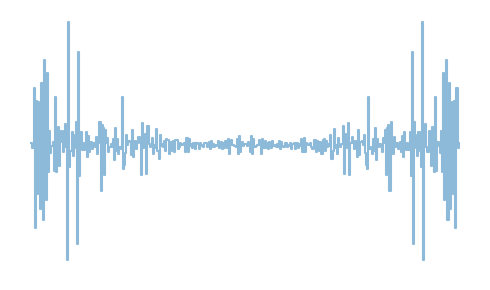
\includegraphics[scale=0.2]{figures/stft2}};
\node[
    left=0.15cm of fft2,
    label={[label distance=-0.25cm]north:{\footnotesize{FFT Output 2}}}
] (fft1) {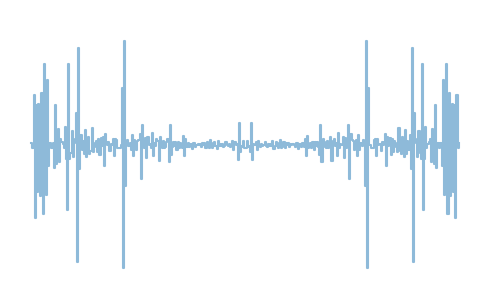
\includegraphics[scale=0.2]{figures/stft1}};
\node[
    left=0.15cm of fft1,
    label={[label distance=-0.25cm]north:{\footnotesize{FFT Output 1}}},
    label={[label distance=0.82cm]west:{\parbox{2.5cm}{\centering \large{Frequency \\ Spectra}}}}
] (fft0) {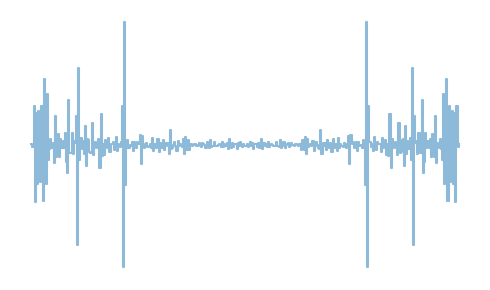
\includegraphics[scale=0.2]{figures/stft0}};

\end{tikzpicture}
    \caption{Application of the \gls{STFT} to a signal. The original waveform is multiplied by multiple offset window functions, producing a set of overlapping signal partitions. The \gls{FFT} is then applied to each partition individually, resulting in a sequence of frequency spectra that preserve localized time–frequency information.}
    \label{STFTFigure}
\end{figure}

The \gls{STFT} has several parameters that affect the structure and resolution of its output; most notably the \textit{window function}, \textit{window length}, and \textit{hop length}. Due to a phenomenon called \textit{spectral leakage}, where spectral information bleeds into other frequencies, a windowing function is applied to each partitioned segment. A common choice is the \textit{Hann window}, illustrated in Figure~\ref{HannWindowFigure}.

The window length plays a crucial role in determining the time–frequency resolution. A longer window improves the frequency resolution, allowing for more precise magnitude estimation of each frequency component, but comes at the cost of reduced time resolution. This is because a large window spans a longer segment of the signal, causing individual windows to overlap more and blur timing information. On the contrary, shorter windows improve temporal precision but blur frequency content, due to each window consequently consisting of fewer samples. This duality is known as the \textit{time–frequency tradeoff}.

The hop length determines how far the window shifts between each segment and directly affects the temporal granularity of the output. A smaller hop length results in more overlap and a finer temporal resolution, but also increases the computational cost by requiring more \glspl{FFT}. Additionally, the hop length defines the time step between frames, allowing each window to be assigned a temporal index.

\begin{figure}[H]
    \centering
    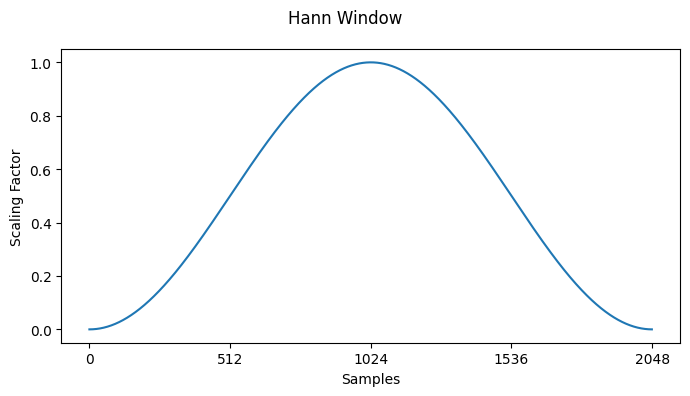
\includegraphics[scale=0.8]{figures/hann}
    \caption{The Hann window function, commonly applied to each partition during the \gls{STFT} to reduce the effects of spectral leakage. It does so by scaling the amplitude of the signal down toward zero at the window's edges. This example shows a window length of 2048 samples.}
    \label{HannWindowFigure}
\end{figure}

For \gls{ADT}, a common configuration is to use the Hann window, with a window size of 2048 samples and a hop length corresponding to 10~ms, i.e., the sampling rate divided by 100~\cite{8350302, vogl2016recurrent,vogl2018multiinstrumentdrumtranscription, signals4040042}.

\subsection{Spectrogram}

The \gls{STFT}, like the standard Fourier Transform, produces complex-valued output. To convert this into strictly real-valued data without discarding meaningful information, we compute the \textit{spectrogram}. Specifically, a magnitude spectrogram is obtained by taking the absolute value of each complex result from the \gls{STFT}.

The result is a two-dimensional, real-valued representation of the signal, where one axis corresponds to time and the other to frequency. While this representation can be modeled as a time series, it is also structurally equivalent to an image. As such, spectrograms are often visualized as heatmaps, offering an intuitive way to observe how frequency information evolves over time.

\begin{figure}[H]
    \centering
    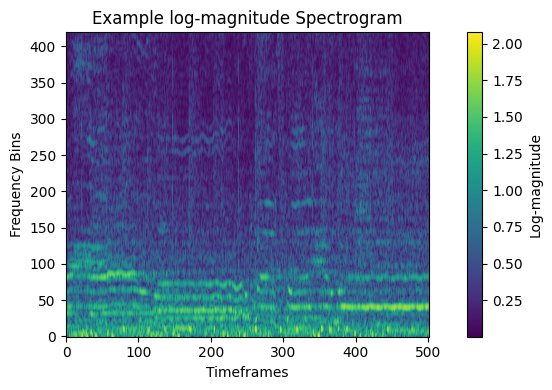
\includegraphics[scale=1.1]{figures/logspectrogram}
    \caption{Log-magnitude spectrogram of the SADTP track \textit{"Red Swan"}, showing the segment from 3:35 to 3:40 minutes. The spectrogram is computed using 2048 \glspl{FFT}, with a window length of 512 samples and a hop length corresponding to 10~ms. Only the first 420 frequency bins are visualized. The color represents the log-magnitude of each time–frequency bin.}
    \label{SpectrogramFigure}
\end{figure}

The number of frequency bins (represented on the y-axis of Figure \ref{SpectrogramFigure}) in a spectrogram is equal to half the number of \glspl{FFT} used in its computation. These bins contain information about linearly spaced frequencies, ranging from 0~Hz up to the Nyquist frequency of the signal. The number of time frames (the x-axis) is determined by the hop length of the \gls{STFT}, with smaller hop lengths resulting in a greater number of frames. In this way, one has significant control over the dimensionality of the spectrogram through parameter selection. 

One drawback of the spectrogram is that it discards all information about signal's phase. As previously mentioned, phase is encoded in the angle of each complex value, which is lost when computing the magnitude. This means it is not possible to perfectly reconstruct the original signal from a magnitude-only spectrogram. However, approximate reconstruction is possible using iterative algorithms such as Griffin–Lim~\cite{1164317}.

\subsection{Loudness of Magnitude}

The human perception of loudness is approximately logarithmic. A soundwave that carries ten times more energy is not perceived as ten times louder. Instead, a doubling in perceived loudness corresponds roughly to a 10~\gls{dB} increase in signal amplitude. The \acrlong{dB} is a relative unit of measurement that expresses the power the ratio between two signals, where an increase of 1~\gls{dB} corresponds to a power ratio of $10^\frac{1}{10}$. The power of a signal is computed as the square of its magnitude. 

This relationship has two major consequences. First, the magnitude scale used in standard spectrograms does not align with human perception of loudness; quiet and loud signals may differ significantly in magnitude, even if they perceptually seem close. Second, this mismatch causes the standard (linear) spectrogram to be highly variable in its magnitude representation, often making it difficult to identify quieter frequency components among louder ones.

To address this, a log-magnitude spectrogram is often used (as in Figure \ref{SpectrogramFigure}), which applies a logarithmic transformation to the magnitudes. This logarithm is typically base 10, aligning with the \acrlong{dB} scale and better reflecting human auditory perception.

\begin{figure}[H]
    \centering
    \hspace*{-1.0cm}
    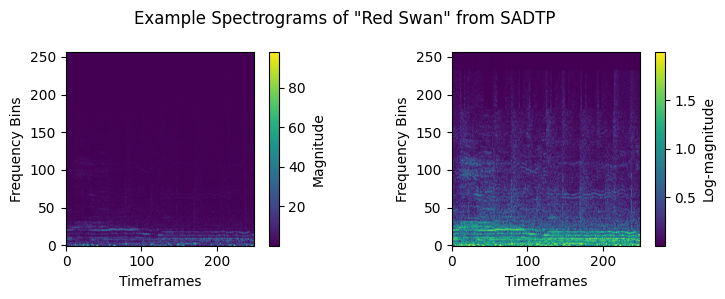
\includegraphics[scale=1.0]{figures/spectrogramlogspectrogram}
    \caption{Comparison between a linear magnitude spectrogram and a log-magnitude spectrogram. When scaled linearly, differences in magnitude are harder to distinguish, especially for quieter frequency components. The logarithmic scale makes both loud and quiet components visually more distinguishable.}
    \label{SpectrogramLogspectrogramFigure}
\end{figure}

\subsection{Filters}

Signal frequencies and human perception have a non-linear relationship. Just as loudness is perceived on a logarithmic scale, so too is pitch. Humans perceive logarithmic differences in frequency as a linear difference in pitch, and are more sensitive to changes in lower frequencies than in higher ones. For example, the notes $\text{A}_2$ and $\text{B}_2$ differ by approximately 13.47~Hz, while $\text{D}_7$ and $\text{E}_7$ differ by nearly 287.70~Hz, yet both are perceived as being one semitone apart, meaning they audibly have the same perceived difference in pitch. Because the frequency bins in a standard spectrogram are spaced evenly in frequency, they do not reflect how pitch is actually perceived, with finer sensitivity in lower regions and coarser sensitivity in higher ones.

To better reflect this, we apply a set of \textit{filters}, each emphasizing a certain frequency range. A filter is typically a triangular weighting function centered at a specific frequency, gradually tapering off toward neighbouring bins. Multiple filters are combined into a \textit{filterbank}, which can be applied to a spectrogram using matrix multiplication. This transforms the frequency axis into a new scale that better aligns with how we hear changes in pitch.

\subsubsection{Mel Spectrograms}

The mel scale, introduced by Stevens, Volkmann, and Newmann in 1937, transforms the frequency axis into a perceptual pitch scale where equal steps correspond to equal perceived pitch differences. In other words, a linear difference in mels is perceived as a linear difference in pitch. Applying a set of triangular mel-filters results in a \textit{mel spectrogram}, a representation widely used in audio-related machine learning tasks. Mel spectrograms have shown successful application in \gls{AMT}.~\cite{gardner2022mt3multitaskmultitrackmusic, chang2024yourmt3+, gong2021astaudiospectrogramtransformer, wolfmonheim2024spectralrhythmfeaturesaudio, 8350302}

\subsubsection{Logarithmic Filters}

While the mel scale was designed to mimic human auditory perception, a different trend has emerged within \acrfull{ADT}. Instead of using perceptual spacing, many recent \gls{ADT} approaches apply \textit{logarithmically spaced filters} centered on the note $\text{A}_4$ (440~Hz), resulting in what is referred to in this thesis as a \textit{logarithmically filtered spectrogram}. 

Unlike mel filters, which are based on models of human hearing, this approach preserves musical structure by spacing filters uniformly on a log-frequency axis. Specifically, it uses 12 filters per octave, corresponding to the 12 semitones in Western music. The filterbank spans the human hearing range, from 20~Hz to 20,000~Hz, and produces a total of 84 frequency bins. Each filter is triangular and area-normalized, meaning that the area under each filter curve equals 1.

This method has been used in several recent \gls{ADT} approaches, particularly by Vogl et al., and has gained traction due to its ability to preserve musically relevant structure while also reducing input dimensionality. It is often favored over mel spectrograms because of its harmonically consistent frequency resolution across octaves~\cite{Vogl2017DrumTV, vogl2018multiinstrumentdrumtranscription, jia2019deep, signals4040042, zehren2024analyzingreducingsynthetictorealtransfer}.

\begin{figure}[H]
    \centering
    \hspace*{-0.6cm}
    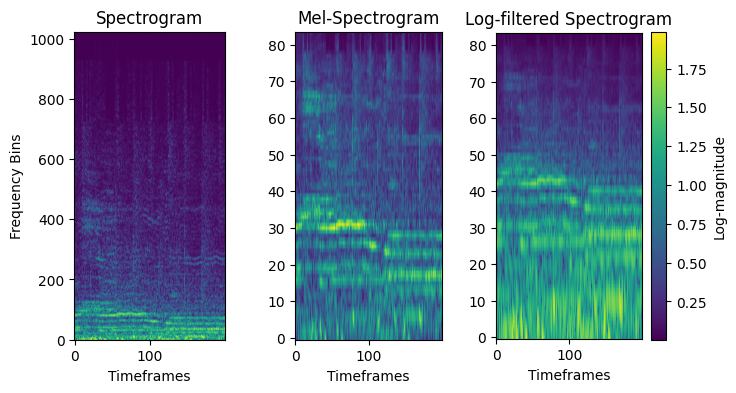
\includegraphics[scale=0.9]{figures/allspectrograms}
    \caption{Comparison between a full log-magnitude spectrogram, a log-magnitude mel spectrogram, and a log-magnitude log-filtered spectrogram. Both the mel and log-filtered spectrograms apply 84 area-normalized filters, resulting in a non-linear frequency axis. While the mel spectrogram emphasizes perceptual resolution with more detail in lower frequencies, the log-filtered spectrogram exhibits uniform resolution across octaves, aligning with musical intervals.}
    \label{AllSpectrogramFigure}
\end{figure}


\section{Transcription}

Transcription refers to a process in which we convert information from an audible format, like music, to another medium. This medium then contains a \textit{description} of said audio. As we focus on a musical context, there are a few notable such mediums.

\subsection{Music Notation}

Modern staff notation is a written transcription for a given instrument, that contains the \textit{recipe} for a musician to play parts of the original recording. This has become the standard way of noting down music, and is used by musicians of many different genres all throughout the world.

Sheet music with this notation is typically descriptively exhaustive, and contain information about musical properties like instrument onsets, tempo, velocity, etc. When reading it, time moves horizontally from left-to-right. Each note represents an onset, where the onset's pitch (for melodic instruments) or percussion (for percussive instruments, like the drum set) is denoted by the note's vertical position. The duration or time segment of a given onset is denoted by the form of the note-head or note-stem.

\begin{figure}[H]
    \centering
    \begin{tikzpicture}

\node[anchor=west] at (0, 0) {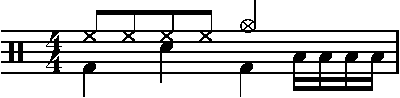
\includegraphics[scale=1.9]{lilypond/drumsheet.cropped.pdf}};

\matrix[
anchor=east,
row sep=-0.205cm
] at (0, 0.1){
    \node[font=\normalsize] {\acrshort{CC+RC}}; \\
    \node[font=\normalsize] {\acrshort{HH}}; \\
    \node[font=\normalsize] {\acrshort{SD}}; \\
    \node[font=\normalsize] {\acrshort{TT}}; \\
    \node[font=\normalsize] {\acrshort{KD}}; \\
};

\end{tikzpicture}
    \caption{An example drum sheet containing all instruments of a 5-instrument \gls{ADT} task. The instrument in each respective row is shown on the left. From the bottom they are the \acrfull{KD}, \acrfull{TT}, \acrfull{SD}, \acrfull{HH}, and \acrfull{CC+RC}.}
    \label{DrumsheetFigure}
\end{figure}

Note that rest marks, like \HaPa, \ViPa, \AcPa, or \SePa, might appear in notation transcriptions. These are symbols which indicate silence or pauses in the music. Although these might appear inline with the instrument onsets, one should not expect an onset at their respective timing, rather it indicating a short break.

\subsection{MIDI Annotations}

\gls{MIDI} is the industry standard for handling music digitally. It is a binary format, containing sequences of commands that allow digital interfaces to \textit{synthesize} music. As it is binary, it is unreadable to us humans without translating it into another format. When computers play \gls{MIDI} arrangements, the \gls{MIDI} sequences are parsed at a constant speed, playing different sounds through \textit{note on}/\textit{note off} events, delayed by time \textit{deltas}. Similar to sheet music, \gls{MIDI} is also very descriptive. And one could say that, intuitively, \gls{MIDI} is to a computer what sheet music is to a musician.

Recently, outputting transcriptions in a \gls{MIDI}-like format has been attempted in \gls{DTM}, and has shown to be promising. Utilizing a sequence-to-sequence \gls{NLP} approach, Gardner et al. presented MT3~\cite{gardner2022mt3multitaskmultitrackmusic}, a model inputting spectrograms and outputting \gls{MIDI} events autoregressively. This format was expanded on by Chang et al.'s YourMT3+~\cite{chang2024yourmt3+}, using a \gls{LLM} instead.

\begin{figure}[H]
    \centering
    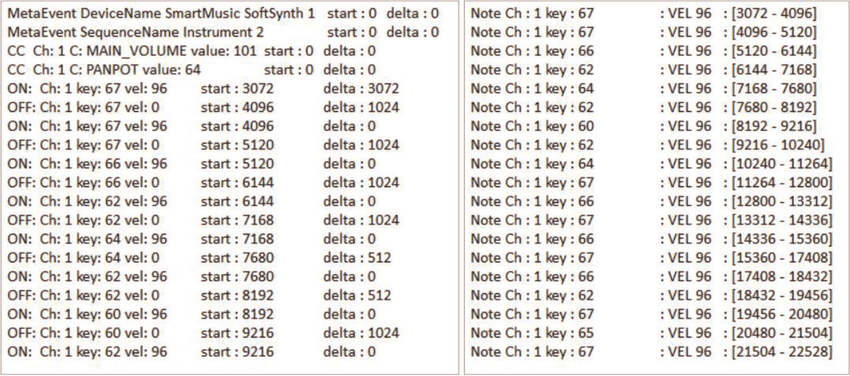
\includegraphics[scale=0.65, trim={0 0 13.8cm 0},clip]{figures/midi}
    \caption{Example MIDI arrangement in text format. The first lines contain meta data. Afterwards follow lines with note on/off events, with temporal information start and delta, with the instrument and sound being decided by channel, key and velocity information~\cite{starostenko2019}.}
    \label{MIDIFigure}
\end{figure}

\subsection{Activation Functions}

In machine learning, the task of detecting instrument onsets could be described as a multi-label sequence labeling task. This involves, for each timeframe in a sequence, predicting a probability, or rather confidence value, that a certain instrument onset happens. In the domain of \gls{MIR} and \gls{AMT}, it has become common place to describe these confidence distributions as \textit{activation functions}; not to be confused with the general deep learning term, activation functions like ReLU or sigmoid.~\cite{8350302, Southall2016AutomaticDT, vogl2018multiinstrumentdrumtranscription}

This way of frame-level prediction is extensively used within onset detection in \gls{ADT} and is the approach we will be taking in this thesis. When predicting these activation functions, we concatenate each activation function distribution rowwise onto a matrix format, based on each instrument.

\begin{figure}[H]
    \centering
    \hspace*{-0.5cm}
    \begin{tikzpicture}

% Drum Sheet
\node[
    anchor=east,
    label=north:{\large{Drum Notation}}
] at (0, 0) {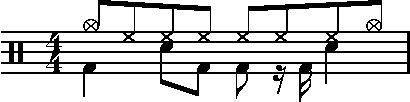
\includegraphics[scale=1.2]{lilypond/activations.cropped.pdf}};


% Activation Functions
\node[
    anchor=south
] at (5, 3.1) {\large{Activation Functions}};

% Cymbals and Ride
\draw[->,
thick
] (0, 0.5) -- (2, 2.5) node[midway, fill=white] {\acrshort{CC+RC}};
\draw[
    anchor=west,
    shift={(2.45, 2.1)}
] (-0.25, -0.1) -- (5.25, -0.1) -- (5.25, 0.9) -- (-0.25, 0.9) -- cycle;
\draw[
    anchor=west,
    color=blue,
    shift={(2.45, 2.1)}
] (-0.25, 0) -- (-0.05, 0) -- (0, 0.8) -- (0.05, 0) -- (4.95, 0) -- (5, 0.8) -- (5.05, 0) -- (5.25, 0);
\foreach \point in {(0, 0.8), (5, 0.8)} {
    \draw[
        color=red,
        shift={(2.45, 2.1)}
    ] \point circle (1.7pt);
}


% Hi-Hat
\draw[->,
thick
] (0, 0.25) -- (2, 1.25) node[midway, fill=white] {\acrshort{HH}};
\draw[
    line width=0.6pt,
    anchor=west,
    shift={(2.45, 0.85)}
] (-0.25, -0.1) -- (5.25, -0.1) -- (5.25, 0.9) -- (-0.25, 0.9) -- cycle;
\draw[
    anchor=west,
    color=blue,
    shift={(2.45, 0.85)}
] (-0.25, 0) -- (0.66, 0) -- (0.71, 0.8) -- (0.76, 0) -- (1.37, 0) -- (1.42, 0.8) -- (1.47, 0) -- (2.09, 0) -- (2.14, 0.8) -- (2.19, 0) -- (2.8, 0) -- (2.85, 0.8) -- (2.9, 0) -- (3.52, 0) -- (3.57, 0.8) -- (3.62, 0) -- (4.23, 0) -- (4.28, 0.8) -- (4.33, 0) -- (5.25, 0);
\foreach \point in {(0.71, 0.8), (1.42, 0.8), (2.14, 0.8), (2.85, 0.8), (3.57, 0.8), (4.28, 0.8)} {
    \draw[
        color=red,
        shift={(2.45, 0.85)}
    ] \point circle (1.7pt);
}


% Snare Drum
\draw[->,
thick
] (0, 0) -- (2, 0) node[midway, fill=white] {\acrshort{SD}};
\draw[
    anchor=west,
    shift={(2.45, -0.4)}
] (-0.25, -0.1) -- (5.25, -0.1) -- (5.25, 0.9) -- (-0.25, 0.9) -- cycle;
\draw[
    anchor=west,
    color=blue,
    shift={(2.45, -0.4)}
] (-0.25, 0) -- (1.37, 0) -- (1.42, 0.8) -- (1.47, 0) -- (4.23, 0) -- (4.28, 0.8) -- (4.33, 0) -- (5.25, 0);
\foreach \point in {(1.42, 0.8), (4.28, 0.8)} {
    \draw[
        color=red,
        shift={(2.45, -0.4)}
    ] \point circle (1.7pt);
}


% Tom-Toms
\draw[->,
thick
] (0, -0.25) -- (2, -1.25) node[midway, fill=white] {\acrshort{TT}};
\draw[
    anchor=west,
    shift={(2.45, -1.65)}
] (-0.25, -0.1) -- (5.25, -0.1) -- (5.25, 0.9) -- (-0.25, 0.9) -- cycle;
\draw[
    anchor=west,
    color=blue,
    shift={(2.45, -1.65)}
] (-0.25, 0) -- (5.25, 0);
\foreach \point in {} {
    \draw[
        color=red,
        shift={(2.45, -1.65)}
    ] \point circle (2pt);
}

% Kick Drum
\draw[->,
thick
] (0, -0.5) -- (2, -2.5) node[midway, fill=white] {\acrshort{KD}};
\draw[
    anchor=west,
    shift={(2.45, -2.9)}
] (-0.25, -0.1) -- (5.25, -0.1) -- (5.25, 0.9) -- (-0.25, 0.9) -- cycle;
\draw[
    anchor=west,
    color=blue,
    shift={(2.45, -2.9)}
] (-0.25, 0) -- (-0.05, 0) -- (0, 0.8) -- (0.05, 0) -- (2.09, 0) -- (2.14, 0.8) -- (2.19, 0) -- (2.8, 0) -- (2.85, 0.8) -- (2.9, 0) -- (3.87, 0) -- (3.92, 0.8) -- (3.97, 0) -- (5.25, 0);
\foreach \point in {(0, 0.8), (2.14, 0.8), (2.85, 0.8), (3.92, 0.8)} {
    \draw[
        color=red,
        shift={(2.45, -2.9)}
    ] \point circle (1.7pt);
}

\end{tikzpicture}
    \caption{The activation function representation for a 5-instrument \gls{ADT} task of a piece written in drum notation. Note how the value of each respective activation function is zero everywhere, except at its onsets, where it is one. The $\SePa$ symbol represents a short, 16th note rest in the \gls{KD} instrument, not an onset.}
    \label{ActivationsFigure}
\end{figure}

\subsubsection{Peak-picking}

When predicting activation functions, we need a separate post-processing step to turn these confidence distributions into onset events. By utilizing a standard \textit{peak-picking} algorithm, we can isolate and enhance peaks in these activation functions, and go from a continuous distribution to a collection of discrete events.

The peak-picking algorithm, introduced in its current form by Böck et al.~\cite{Bck2012EvaluatingTO}, defines that a prediction $\hat{y}_n$ at timeframe $n$ is a \textit{peak} if it fulfills the three conditions:
\begin{align*} 
    \hat{y}_n &= \text{max}(\hat{y}_{n - m}, ..., \hat{y}_n, ... \hat{y}_{n + m}), \\ 
    \hat{y}_n &\ge \text{mean}(\hat{y}_{n - a}, ..., \hat{y}_n, ... \hat{y}_{n + a}) + \delta, \\
    n &\ge n_\text{last onset} + w.
\end{align*}

For appropriately trained deep learning models, Vogl et al.~\cite{vogl2018multiinstrumentdrumtranscription} showed that the peak-picking parameters which gave the best results were $m = a = w = 2$ and $\delta = 0.1$. Consequently, these same parameter values are applied for this thesis.


\section{Automatic Drum Transcription}

\textcolor{red}{This whole section and the two other following need to be rewritten after moving them. Shouldn't be too big of an issue.}

As mentioned, \gls{ADT} describes the task of transcribing symbolic notation for drums from audio. To be even more descriptive, \gls{ADT} can be split into further tasks. From least to most complex we have: \gls{DSC}, where we classify drum instruments from isolated single event recordings. \gls{DTD}, where we transcribe audio containing exclusively drum instruments. \gls{DTP}, where we transcribe audio containing drum instruments, and additional percussive instruments which the transcription should exclude. Finally, we have \gls{DTM}, which describes the task of drum transcription with audio containing both drum, and melodic instruments.~\cite{8350302}

As mentioned, this thesis will focus on the most complex of these, namely \gls{DTM}. Intuitively, we want to develop a deep learning model which, given input audio, has the ability to detect and classify different drum instrument onsets (events), while selectively ignoring unrelated, melodic instruments.

This task comes with difficulties not seen in the less complex tasks. Zehren et al.~\cite{signals4040042} describes one example, in where \textit{"melodic and percussive instruments can overlap and mask eachother..., or have similar sounds, thus creating confusion between instruments"}.

Deep learning has shown to be a promising method to solve such a task, and several different approaches have been tried, many with great success. Vogl et al.~\cite{vogl2018multiinstrumentdrumtranscription, Vogl2017DrumTV} displayed good results with both a convolutional, and a convolutional-recurrent neural network. Zehren et al.~\cite{signals4040042, zehren2024analyzingreducingsynthetictorealtransfer} focused on datasets, showing that the amount of data and quality of data are equally important to get good performance. Most recently, Chang et al.~\cite{chang2024yourmt3+} explored an autoregressive, language model approach. This approach explored multi-instrument transcriptions, but their results regarding \gls{DTM} were notable.

This reinforces the fact that there still exist many approaches to attempt, which could lead to a general improvement for both general \gls{ADT} and \gls{DTM} models.

\section{The Drum Set}

The drum set is a collection of percussive instruments like different drums, cymbals, and possibly different auxillary percussions. A drum set can vary in what it is composed of, however a standard kit usually consists of a \gls{SD}, a \gls{KD}, one or more \glspl{TT} (toms), one or more cymbals (\gls{CC} and \gls{RC}), and a \gls{HH} cymbal~\cite{TheDrumHandbook2003}.

\begin{figure}[H]
    \centering
    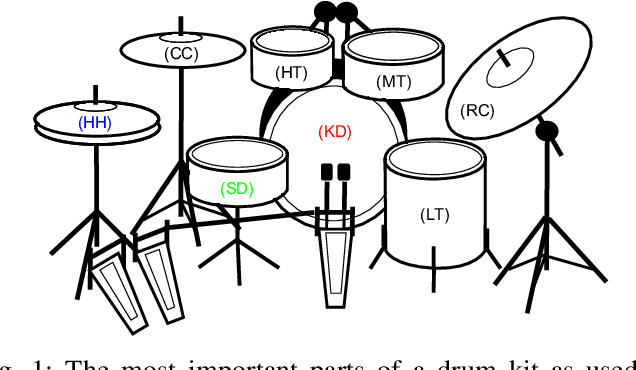
\includegraphics[scale=0.7, trim={0 1cm 0 0},clip]{figures/drumset}
    \caption{Example of the different instruments that make up the full standard drum set. They are the \acrfull{KD}, \acrfull{SD}, \acrfull{HH}, \acrfull{CC}, \acrfull{RC}, \acrfull{HT}, \acrfull{MT}, \acrfull{LT}~\cite{8350302}.}
    \label{DrumsetFigure}
\end{figure}

As mentioned, percussion like the drum set, stands in contrast to other musical instruments in that the different ways of playing the same instrument often differ a lot in their \textit{"audible footprint"}. The snare drum, bass drum and hi-hat all have quite different timbres, frequency span, volume, and all in all fundamentally are different instruments.

\begin{figure}[H]
    \centering
    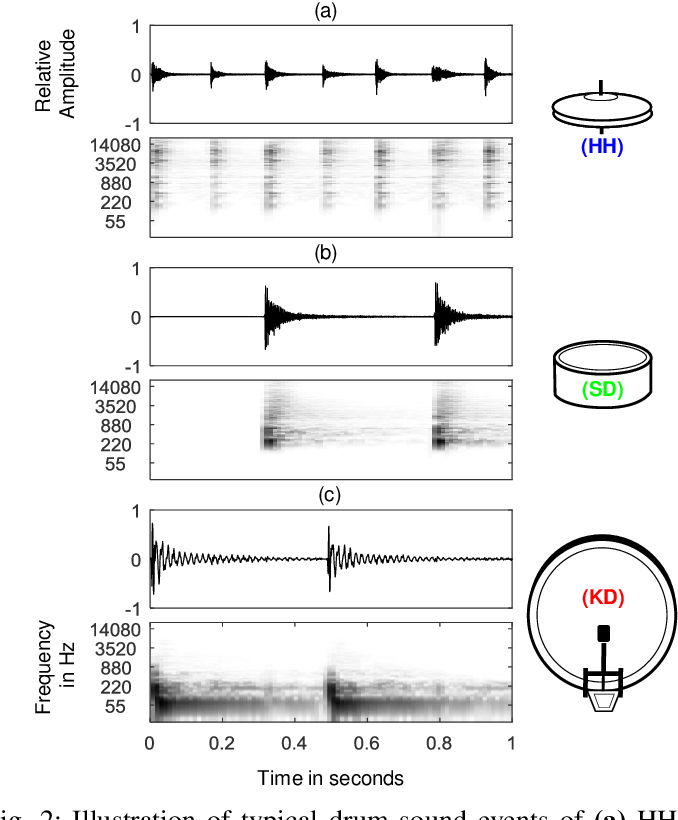
\includegraphics[scale=0.6, trim={0 1cm 0 0},clip]{figures/drumsettimbre}
    \caption{Example of the different audible footprint for drum set percussion. Plotted are the waveforms of three different drum instruments played at different speeds, together with its corresponding spectrogram. The panels show each instrument's time-domain waveform signal, with a corresponding spectrogram below. As we can see, each instrument's event differ in how they look and affect both the waveform and spectrogram~\cite{8350302}.}
    \label{DrumsetTimbreFigure}
\end{figure}

\section{Transcription Task}

Understand the pipeline for a transcription task, specifically \gls{ADT}, is crucial for this thesis. It all starts with an initial audio waveform representing the audio track we want to transcribe, usually split into smaller non-overlapping partitions~\cite{vogl2018multiinstrumentdrumtranscription, gardner2022mt3multitaskmultitrackmusic}. This is parsed into a spectrogram, which unravels the frequencies of the audio wave while condensing information across time, making the input features easier for a model to handle and interpret. The spectrogram is then input into an \gls{ADT} model, such as a \gls{DNN}, which reads this input spectrogram and for each timeframe predicts the probability that a certain instrument is played. These continuous likelihood predictions are then postprocessed into a more readable and intended format, such as drum notation.

\begin{figure}[H]
    \centering
    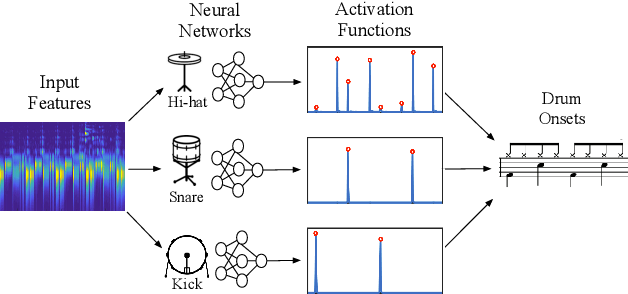
\includegraphics[scale=0.7]{figures/adtpipeline.png}
    \caption{Example of what the prediction pipeline of an \gls{ADT} model could look like. Given an input spectrogram, a model predicts a likelihood distribution of each instrument appearing (called the activation functions), which then is quantized into drum onsets and sheet music notation~\cite{Southall2016AutomaticDT}.}
    \label{ADTFigure}
\end{figure}

Following this pipeline there are certain parameters which need to be kept in mind when constructing the \gls{DNN}, namely: what does the input and ouput of model look like? The input is given as a spectrogram, but these can vary in size and format based different parameters. These will be discussed further in a later section. The output of the model has a sequence size based on the input spectrogram, but also based on the number of instruments we want to transcribe.

Early \gls{ADT} literature used a 3-instrument approach, predicting the basic \acrfull{KD}, \acrfull{SD} and \acrfull{HH}~\cite{vogl2016recurrent}. These give a useful basis in investigating wether \gls{ADT} problems are solvable using deep learning methods, but are too sparse as this leaves out instruments crucial to the basic drum set. To address this, we expand to a 5-instrument approach, including cymbals (capturing both \acrfull{CC} and \acrfull{RC}) and \acrfull{TT} (capturing all toms) in addition to the three prior instruments. This makes the problem slightly more complex, but allows for denser coverage by representing the standard, full drum set.


\section{Performance Measure}

\subsection{Correct Predictions}

Our machine learning models predict instrument onset events on a frame-level basis. In other words, are predictions are very granular, and we need some way to decide when a prediction is correct versus incorrect. In \gls{ADT}, a standard has become to allow a \textit{tolerance window} where event predictions are correct if they lie within a certain time window, often between $25\text{ms}$ and $50\text{ms}$. A side effect of this is that, by shifting our focus to predicted events, we lose information about \textit{not} predicting any events~\cite{vogl2016recurrent}.

\subsection{Accuracy}

For classification tasks, a standard performance measure would be \textit{accuracy}: \[ \text{Accuracy} = \frac{\text{TP} + \text{TN}}{\text{TP} + \text{TN} + \text{FP} + \text{FN}}.\] Summing up correct predictions, \gls{TP} and \gls{TN}, and dividing by total number of predictions, sum of \gls{TP}, \gls{TN}, \gls{FP} and \gls{FN}, we find a model's probability of having a correct prediction.

This performance measure falls short in that it is very susceptible to imbalanced datasets. In \gls{ADT}, most timeframes contain no onset, meaning a naïve predictor would get a high accuracy by never predicting any onsets. Another problem with accuracy is that, due to our tolerance window approach we do not necessarily have quantities for \gls{TN}, such that the standard accuracy computation would be incomputable.

\subsection{F1-score}

Mentioned above are some of the reasons why \textit{F1-score} has become the typical performance measure within \gls{ADT}. F1-score combines and tries to maximize two different performance measures, namely \textit{precision}; \[ \text{Precision} = \frac{\text{TP}}{\text{TP} + \text{FP}}, \] and \textit{recall}; \[ \text{Recall} = \frac{\text{TP}}{\text{TP} + \text{FN}}. \]

The precision of a model can tell us how good it is at \textit{hitting} predictions. \textit{Perfect precision} happens when a model has no \gls{FP}, i.e. never predicting an event where one doesn't happen. Recall is similar, but represents the other end of the stick. It tells us how good a model is at \textit{not missing} predictions. \textit{Perfect recall} happens when a model has no \gls{FN}, i.e. never \textit{not} predicting an event where one does happen.

As mentioned, F1-score combines these two measures in an aggregate performance measure by computing their harmonic mean: $$ \text{F1-score} = \frac{2 \cdot \text{Precision} \cdot \text{Recall}}{\text{Precision} + \text{Recall}}. $$ By maximizing F1, we simultaneously maximize both precision and recall as well, reaping all their benefits.

\subsection{Micro vs. Macro}

There are different ways of computing and combining F1-score on multi-label data. Even though they might seem similar, they fundamentally represent different information, and thus the choice in which one to select is crucial.

\textit{Macro F1-score} is computed through the arithmetic mean of the classwise computed F1-scores. Finding a model which maximizes this measure would be similar to finding the model which performes best on each of the separate classes, preventing a class from taking priority due to imbalanced datasets. Relating this to \gls{ADT}, it would mean focusing on transcribing each instrument equally well.

\textit{Micro F1-score} is computed through finding the F1-score with global \gls{TP}, \gls{FP}, \gls{FN} values. Maximizing this would mean prioritizing classes that occur more frequently in the datasets. Such as in \gls{ADT}, this would mean focusing on transcribing instruments which appear often, like the snare or base drum, over rarer instruments like the toms.

For \gls{ADT}, the trend has been to select Micro F1-score as the main performance measure, due to its ability to show a model's \textit{general} performance on musical pieces. We want our model to maximize their ability to transcribe music, not maximize their ability to transcribe each instrument in said music. \gls{ADT}, prioritizing frequent instruments is relevant. As mentioned previously, the more frequent instruments lay the ground work for the fundamentals, and could be said to be more important than scarcely occuring ones.

\begin{figure}[H]
    \centering
    \hspace*{-0.5cm}
    \begin{tikzpicture}
    
% True Transcription
\node[
    anchor=east,
    label=north:{\large{True Transcription}}
] (true) at (0, -0.5cm) {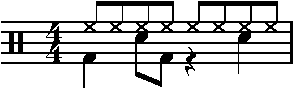
\includegraphics[scale=1.2]{lilypond/example_label.cropped.pdf}};

% Predicted Transcription
\node[
    anchor=west,
    label=north:{\large{Predicted Transcription}}
] (pred) at (0, -0.5cm) {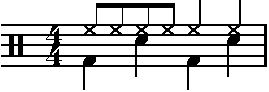
\includegraphics[scale=1.2]{lilypond/example_prediction.cropped.pdf}};


% False Positives
\node[
    anchor=north,
    label={[label distance=0.49cm]north:{\normalsize{\acrfullpl{FP}}}},
] (fp) at (0, -3cm) {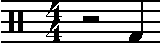
\includegraphics[scale=1.2]{lilypond/example_fp.cropped.pdf}};

% True Positives
\node[
    anchor=north,
    label=north:{\normalsize{\acrfullpl{TP}}},
    left=0.25cm of fp
] {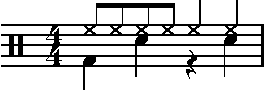
\includegraphics[scale=1.2]{lilypond/example_tp.cropped.pdf}};
    
% False Negatives
\node[
    anchor=north,
    label={[label distance=0.49cm]north:{\normalsize{\acrfullpl{FN}}}},
    right=0.25cm of fp
] {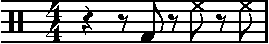
\includegraphics[scale=1.2]{lilypond/example_fn.cropped.pdf}};

\matrix[
    column sep=0.5cm
] at (0, -5cm) {
    \node {\large{\textbf{Classwise F1}:}}; &
    \node[
        label=north:{\large{\acrshort{KD}}}
    ] {\large{0.5}}; &
    \node[
        label=north:{\large{\acrshort{SD}}}
    ] {\large{1.0}}; &
    \node[
        label=north:{\large{\acrshort{HH}}}
    ]{\large{0.86}}; \\
};
\matrix[
    column sep=0.5cm
] at (0, -6cm) {
    \node {\large{\textbf{Macro F1}: 0.79}}; &
    \node {\large{\textbf{Micro F1}: 0.82}}; \\
};


\end{tikzpicture}
    \caption{Example of computing the different F1-scores of from a true and predicted \gls{ADT} transcription. The \HaPa, \ViPa, or \AcPa symbols represent pauses, and not instrument onsets. Note how the Macro F1 better represents the F1-score of all individual instruments, where as Micro F1 better represents the F1-score of the transcription as a whole. For readability, F1-scores are written with a precision of two decimals.}
    \label{F1Figure}
\end{figure}